In order to navigate, a model of the environment is required. This model is stored in the Environment Descriptor (\acrshort{ed}). From this model, a planning representation is derived that enables using the model of the environment for navigation purposes.
\begin{figure}[ht]
	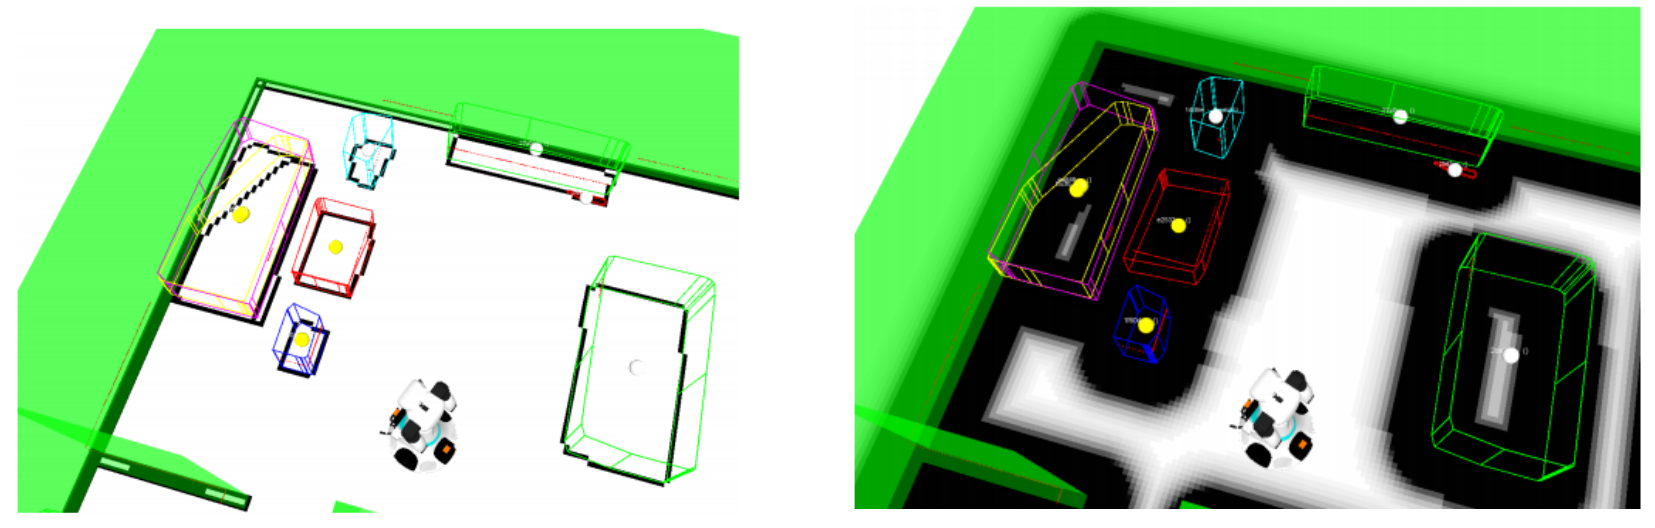
\includegraphics[width = \linewidth]{Figures/ed_navigation}
	\caption{Grid representation of the environment.}
	\label{fig:ed_navigation}
\end{figure}
With use of the ed\_navigation plugin \footnote{\url{https://github.com/tue-robotics/ed_navigation}}, an occupancy grid is derived from the world model and published as a nav\_msgs/OccupancyGrid, as illustrated in the picture above. This representation can be used by a motion planner to perform searches in the configuration space of the robot.
\\\\
An example of such a motion planner is move\_base\footnote{\url{http://wiki.ros.org/move_base}} or the cb\_base\_navigation\footnote{\url{https://github.com/tue-robotics/cb_base_navigation}} ROS package. The latter software package, in contradiction to the move\_base software package is able to deal with end goal constraints. With use of a ROS service, provided by the ed\_navigation plugin, an end goal constraint can be constructed w.r.t. a specific world model entity described by ED. This enables the robot to not only navigate to poses but also to areas or entities in the scene, as illustrated by the following picture.
\begin{figure}[ht]
	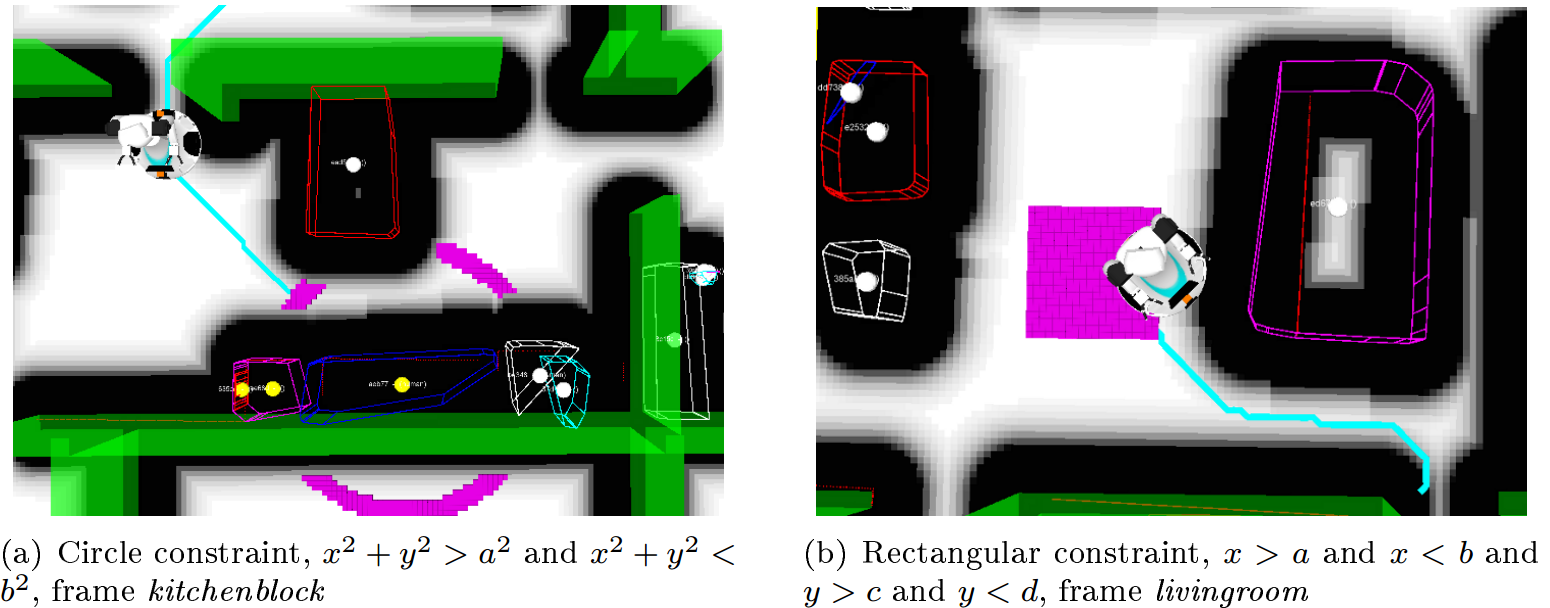
\includegraphics[width = \linewidth]{Figures/ed_navigation_constraints}
	\caption{Navigation position constraints w.r.t. other entities in the environment}
	\label{fig:ed_navigation_constraints}
\end{figure}
As for the local and global motion planners, somewhat modified versions of the ROS planners available within move\_base are used.
The configurations for move\_base node has now been created for the AMIGO and SERGIO robots, the HSR node will be added. The node integrates local and global path planning and local control. Its actionlib interface has become in fact standard for sending 2D navigation goals to robots in ROS. 